% !TEX root = ../thesis-sample.tex

\chapter{STANDARD MODEL} \label{chap:intro}



\section{Basic concepts}

 %%%% Teoria    2 semanas  %%%%%%%%%%%%%
 
 %%%%%%%  En paralelo
%%%%%%%%  a) Finalizar implemntacion de script para generacion de muestras en ACARUS, subir al github archivo python  
%%         b) Producir los grafficos de parametrizacion de eficiencia y resolucion de mmuones que delphes usa   delphes_card_CMS.tcl 
%%        
There are four fundamental forces at work in the universe: the strong force, the weak force, the electromagnetic force, and the gravitational force. The Standard Model includes the electromagnetic, strong and weak forces and all their carrier particles, and explains well how these forces act on all of the matter particles.

\subsection{Fundamental forces}

The fundamental forces (or fundamental interactions) of physics are the ways that individual particles interact with each other. It turns out that every single interaction observed taking place in the universe can be broken down and described by only four (well, generally four—more on that later) types of interactions:

\begin{itemize}
    \item \textbf{\textcolor{azul50}{Gravity: }} has the farthest reach, but it's the weakest in actual magnitude. It is a purely attractive force which reaches through even the "empty" void of space to draw two masses toward each other. Is described under the theory of general relativity, which defines it as the curvature of spacetime around an object of mass. This curvature, in turn, creates a situation where the path of least energy is toward the other object of mass.
    \item \textbf{\textcolor{azul50}{Electromagnetism :}} is the interaction of particles with an electrical charge. Charged particles at rest interact through electrostatic forces, while in motion they interact through both electrical and magnetic forces, is the most prevalent force in our world, as it can affect things at a reasonable distance and with a fair amount of force.
    \item \textbf{\textcolor{azul50}{Weak Interaction (or Weak Nuclear Force) :}} is a very powerful force that acts on the scale of the atomic nucleus. It causes phenomena such as beta decay. It has been consolidated with electromagnetism as a single interaction called the "electroweak interaction.", is mediated by the W boson (there are two types, the W+ and W- bosons) and also the Z boson.
    \item \textbf{\textcolor{azul50}{Strong Interaction (or Strong Nuclear Force) :}} the strongest of the forces is, keeps the nucleons (protons and neutrons) bound together. In the helium atom, for example, it is strong enough to bind two protons together even though their positive electrical charges cause them to repulse each other, the strong interaction allows particles called gluons to bind together quarks to create the nucleons in the first place. Gluons can also interact with other gluons, which gives the strong interaction a theoretically infinite distance, although it's major manifestations are all at the subatomic level.
\end{itemize}


\subsection{Particle Families}

Fundamental particles are either the building blocks of matter, called fermions, or the mediators of interactions, called bosons. Every elementary particle has associated with it a spin quantum number $s$ (often called the spin number or just the spin), where $s$ is any whole number multiple of a half. Fermions have half integral spin quantum numbers ($1/2$, $3/2$, $5/2$, etc.) and bosons have integral spin quantum numbers ($0$, $1$, $2$, etc.). No spin numbers are possible in between these. 

\begin{figure}
    \centering
    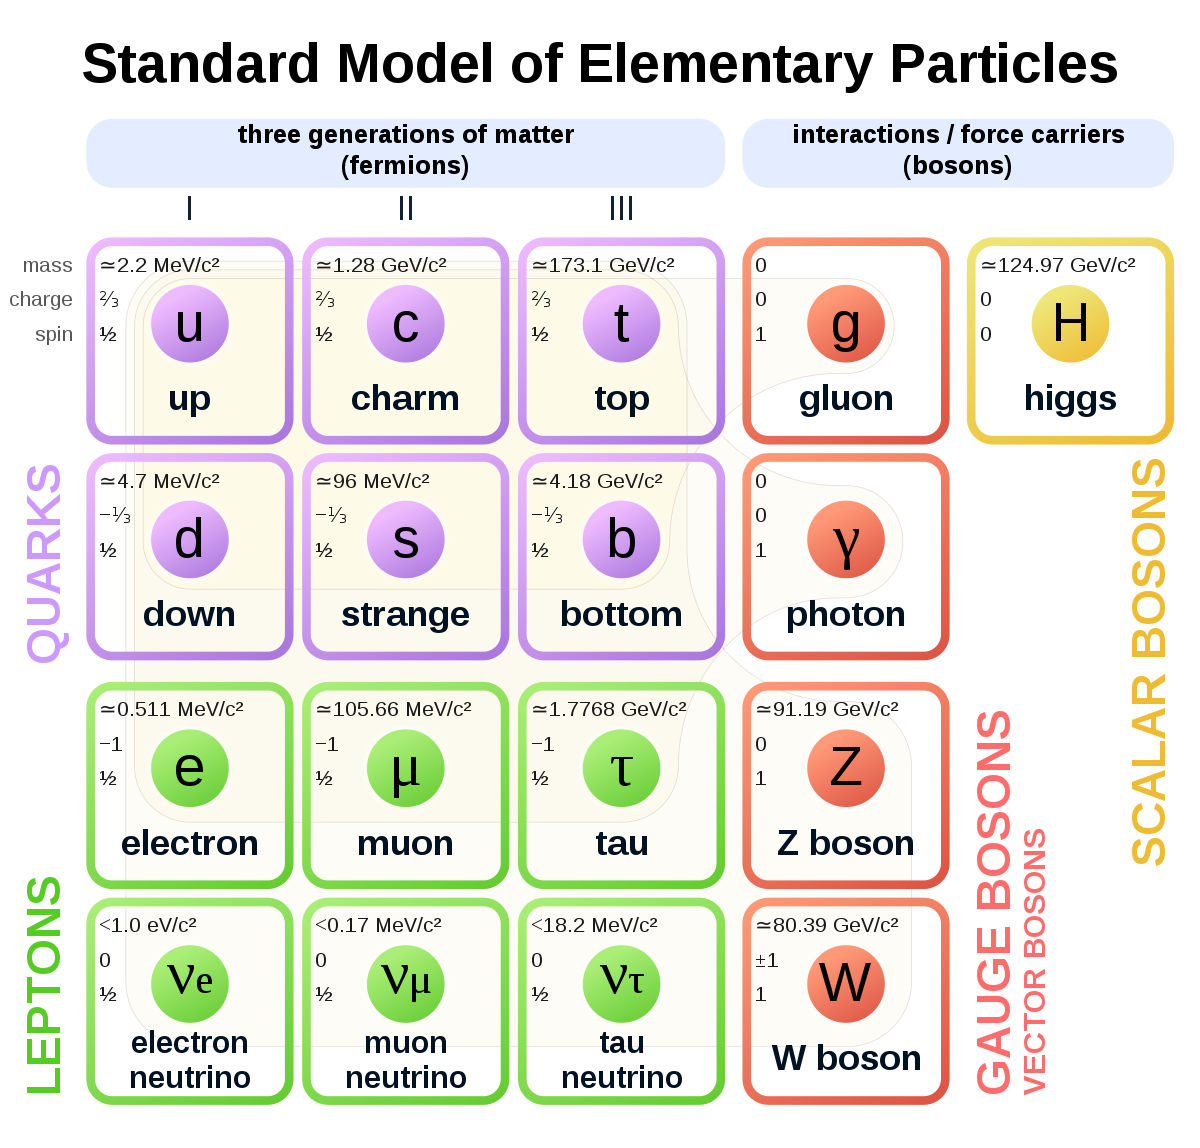
\includegraphics[width=0.7\textwidth]{tex/Chapters/Standard_Model/Imagen/Model.png}
    \caption{Standard model particles.}
    \label{fig:estandard_model}
\end{figure}

Fermions obey a statistical rule described by Enrico Fermi (1901–1954) of Italy, Paul Dirac (1902–1984) of England, and Wolfgang Pauli (1900–1958) of Austria called the exclusion principle. Simply stated, fermions cannot occupy the same place at the same time. (More formally, no two fermions may be described by the same quantum numbers.) Leptons and quarks are fermions, but so are things made from them like protons, neutrons, atoms, molecules, people, and walls. This agrees with our macroscopic observations of matter in everyday life. People cannot walk through walls unless the wall gets out of the way.

Bosons, in contrast, are have no problem occupying the same place at the same time. (More formally, two or more bosons may be described by the same quantum numbers.) The statistical rules that bosons obey were first described by Satyendra Bose (1894–1974) of India and Albert Einstein (1879–1955) of Germany. Gluons, photons, and the W, Z and Higgs are all bosons. As the particles that make up light and other forms of electromagnetic radiation, photons are the bosons we have the most direct experience with. In our everyday experience, we never see beams of light crash into one another. Photons are like phantoms. They pass through one another with no effect.

%All fundamental and composite particles have a spin quantum number s (lowercase). This is associated with a spin angular momentum S (uppercase). The SI unit of angular momentum is the kilogram meter squared per second [kgm2/s] or, equivalently, the joule second [Js], which is much too large for elementary particles. Instead ℏ (h bar), also known as the reduced Planck constant (ℏ = h/2π), is used. For reasons that are beyond the scope of this book, the spin quantum number s (which is just a number) and the spin angular momentum S (which is a number with a unit) are not numerically the same. Instead, they are related by a non-obvious equation.


\begin{table}[h!]
  \begin{center}
    \caption{Standard model particles.}
    \label{tab:table1}
    \begin{tabular}{|c|c|c|c|c|c|c|c||} 
        \hline\hline
        \multicolumn{3}{|c|}{\textbf{Family}} & \textbf{Particle} & \textbf{Spin Number} & \textbf{Charge (e)} & \textbf{Color} & \textbf{Mass}\\
        \hline
        F & Q & $u$ & Up Quarks & $1/2$ & $+2/3$ & $r, g, b$	& $2.16$ \\
        \hline
        E & U & $d$ & Down Quark & $1/2$ & $-1/3$ & $r, g, b$ & $4.67$ \\ 
        \hline
        R & A & $c$ & Charm Quark & $1/2$ & $+2/3$ & $r, g, b$ & $1,27$ \\
        \hline
        M & R & $s$ & Strange Quark & $1/2$ & $-1/3$ & $r, g, b$ & $93$ \\
        \hline
        I & K & $t$ & Top Quark & $1/2$ & $+2/3$ & $r, g, b$ & $172.9$ \\
        \hline
        O &  & $b$ & Bottom Quark & $1/2$ & $-1/3$ & $r, g, b$ & $4.18$ \\
        \hline
        N & L & $e$ & Electron & $1/2$ & $-1$ & none & $\approx 0.51$ \\
        \hline
        S & E & $\mu$ & Muon & $1/2$ & $-1$ & none & $\approx 105.65$ \\
        \hline
          & P &  $\tau$ & Tau & $1/2$ & $-1$ & none & $1776.86$ \\
        \hline
          & T & $v_e$ & Electron Neutrino & $1/2$ & $0$ & none & $<2\times10^{-6}$ \\
        \hline
          & O & $v_\mu$ & Muon Neutrino  & $1/2$ & $0$ & none & $<0.19$ \\
        \hline
          & N & $v_\tau$ & Tau Neutrino & $1/2$ & $0$ & none & $<1.2$ \\
        \hline
          & $-$ & $p$ & Proton & $1/2$ & $+1$ & none & $\approx 938.27$ \\
        \hline
          & $- $& $n$ & Neutron & $1/2$ & $0$ & none & $\approx 939.56$ \\
        \hline
        B & & $g$ & Gluon & $1$ & $0$ & 8 colors & $0$ \\
        \hline
        O & & $\gamma$ & Photon & $1$ & $0$ & none & $0$ \\
        \hline
        S & & $W$ & W Boson & $1$ & $0$ & none & $0$ \\
        \hline
        O & & $Z$ & Z Boson & $1$ & $0$ & none & $0$ \\
        \hline
        N & & $H$ & Higgs Boson & $0$ & $0$ & none & $125.1$ \\
        \hline
        \end{tabular}
  \end{center}
\end{table}

Elementary particles have an intrinsic spin angular momentum $S$. The adjective intrinsic means innate or essential to the thing itself. Elementary particles don't have spin because someone is spinning them. They just spin — or rather, they just have a measurable quantity with the same units as angular momentum. In current physics, elementary particles are featureless — like a mathematical point. In order for something to be perceived as spinning, the thing spinning would need something like a "front" and a "back". Featureless, point particles don't have anything like that. Particle physics is best described with mathematics. Spin is a convenient label for a measurable quality and not a description of reality.


\section{Description of standard model}

The standard model is the name given in the 1970s to a theory of fundamental particles and how thea
\subsection{The elements of the Lagrangian}

The Standard Model of particle physics is a quantum field theory. Therefore, its fundamental elements are quantum fields and the excitations of these fields are identified as particles. For example, the quantised excitation of the electron field is interpreted as an electron. From our viewpoint, it is not only permissible, but even advisable to speak directly of elementary particles instead of field excitations when discussing basic principles of particle physics qualitatively in high school.

The Lagrangian of the standard model is an extremely compact notation. Theoretical particle physicists normally know when to sum over which indices, what different abbreviations and derivatives mean, and when to consider each of the fundamental interactions:
\begin{equation}
    \mathcal{L} = - \dfrac{1}{4}F_{\mu v}F^{\mu v} + i\vec{\psi}{\not D} \psi + \psi_i  Y_{ij} \psi_j \phi + |D_m \phi|^2 - V(\phi)
\end{equation}
n the physics classroom, however, it is very difficult to achieve a deep-level understanding because the required mathematics skills go far beyond high-school level.

$\mathcal{L}$  stands for the Lagrangian density, which is the density of the Lagrangian function L in a differential volume element. In other words, $\mathcal{L}$  is defined such that the Lagrangian L is the integral over space of the density: $L={\int}^{}{{\text{d}}^{3}}x~\mathcal{L}$ . 
In 1788, Joseph–Louis Lagrange introduced Lagrangian mechanics as a reformulation of classical mechanics. It allows the description of the dynamics of a given classical system using only one (scalar) function L=T-V where T is the kinetic energy and V the potential energy of the system. The Lagrangian is used together with the principle of least action to obtain the equations of motion of that system in a very elegant way.

When handling quantum fields, instead of the discrete particles of classical mechanics, the Lagrangian density describes the kinematics and dynamics of the quantum system. Indeed, the Lagrangian density of quantum field theory can be compared to the Lagrangian function of classical mechanics. Hence, it is common to refer to $\mathcal{L}$  simply as 'the Lagrangian'.

The term $-\dfrac{1}{4}F_{\mu v}F^{\mu v}$ is the scalar product of the field strength tensor ${{F}_{\mu \nu}}$  containing the mathematical encoding of all interaction particles except the Higgs boson, where $\mu$ and $v$ are Lorentz indices representing the spacetime components. It contains the necessary formulation for these particles to even exist, and describes how they interact with each other. The contents differ depending on the properties of the interaction particles. For example, photons, the interaction particles of the electromagnetic interaction, cannot interact with each other, because they have no electric charge. Therefore, the contribution of the electromagnetic interaction consists only of a kinetic term, the basis for the existence of free photons. The description of gluons and the weak bosons also includes interaction terms in addition to the kinetic terms. Gluons, for example, are colour-charged themselves and can therefore also interact with each other. This leads to an exciting consequence: the Standard Model of particle physics predicts the existence of bound states consisting only of gluons, so-called 'glueballs'. However, no experiment has detected glueballs thus far.


The term $i\vec{\psi}{\not D} \psi$ describes how interaction particles interact with matter particles. The fields $\psi$ and $\bar{\psi}$  describe (anti)quarks and (anti)leptons. The bar over $\bar{\psi}$  means that the corresponding vector must be transposed and complex-conjugated; a technical trick to ensure that the Lagrangian density remains scalar and real. ${\not D}$  is the so-called covariant derivative, featuring all the interaction particles (except the Higgs), but this time without self-interactions.

The beauty of this term is that it contains the description of the electromagnetic, weak, and strong interactions. Indeed, while all three fundamental interactions are different, the basic vertices by which they can be visualised look quite similar. We will start by discussing the most important interaction of our daily lives, the electromagnetic interaction. Here, pair production or annihilation of electrons and positrons, and the absorption or emission of photons by electrons, are prominent examples. All four of these processes can be represented using Feynman diagrams with the same basic vertex.

This term $\psi_i  Y_{ij} \psi_j \phi$ describes how matter particles couple to the Brout–Englert–Higgs field phgr and thereby obtain mass. The entries of the Yukawa matrix yij represent the coupling parameters to the Brout–Englert–Higgs field, and hence are directly related to the mass of the particle in question. These parameters are not predicted by theory, but have been determined experimentally.

Parts of this term still cause physicists headaches: it is still not clear why neutrinos are so much lighter than other elementary particles, in other words, why they couple only very weakly to the BEH field. In addition, it is still not possible to derive the entries of the Yukawa matrix in a theoretically predictive way.

It is known that particles with high mass, in other words with a strong coupling to the Brout–Englert–Higgs field,also couple strongly to the Higgs boson. This is currently being verified experimentally at the LHC, where Higgs bosons are produced in particle collisions. However, Higgs bosons transform into particle–antiparticle pairs after about 10-22 s. Depending on their mass, i.e. their coupling parameter,certain particle–antiparticle pairs are much more likely, and thus easier to observe experimentally, than others.nThis is because the coupling parameter, which describes the coupling to the Higgs boson, is simply the mass of the particle itself. The Higgs boson is thus more likely to be transformed into pairs of relatively more massive particles and anti-particles. Measurements by the ATLAS detector show, for example, evidence of the direct coupling of the Higgs boson to tauons.

The term $|D_m \phi|^2$ describes how the interaction particles couple to the BEH field. This applies only to the interaction particles of the weak interaction, which thereby obtain their mass. This has been proven experimentally, because couplings of W bosons to Higgs bosons have already been verified. Photons do not obtain mass by the Higgs mechanism, whereas gluons are massless because they do not couple to the Brout–Englert–Higgs field.

The term $V(\phi)$ describes the potential of the BEH field. Contrary to the other quantum fields, this potential does not have a single minimum at zero but has an infinite set of different minima. This makes the Brout–Englert–Higgs field fundamentally different and leads to spontaneous symmetry-breaking (when choosing one of the minima). As discussed for terms 4 and 6, matter particles and interaction particles couple differently to this 'background field' and thus obtain their respective masses. This also describes how Higgs bosons couple to each other. The Higgs boson, the quantised excitation of the BEH field, was experimentally confirmed at CERN in 2012. In 2013, François Englert and Peter Higgs were awarded the Nobel Prize in Physics for the development of the Higgs mechanism.













\section{Experiment CMS}
The Compact Muon Solenoid is a general-purpose particle physics experiment, designed to see a wide range of particles and phenomena produced in LHC collisions. These scientists will use the data collected from the complex CMS detector to search for new phenomena including the Higgs boson, supersymmetry, and extra dimensions. They will also measure the properties of previously-discovered quarks and bosons with unprecedented precision, and be on the lookout for completely new, unpredicted phenomena.

\subsection{Compact Muon Solenoid}

The Compact Muon Solenoid (CMS) experiment is one of two large general-purpose particle physics detectors built on the Large Hadron Collider (LHC) at CERN in Switzerland and France. The goal of CMS experiment is to investigate a wide range of physics, including the search for the Higgs boson, extra dimensions, and particles that could make up dark matter.

CMS is 21 metres long, 15 m in diameter, and weighs about 14,000 tonnes, is designed as a general-purpose detector, capable of studying many aspects of proton collisions at 0.9-13 TeV, the center-of-mass energy of the LHC particle accelerator.

The CMS detector is built around a huge solenoid magnet. This takes the form of a cylindrical coil of superconducting cable that generates a magnetic field of 4 teslas, about 100 000 times that of the Earth. The magnetic field is confined by a steel 'yoke' that forms the bulk of the detector's weight of 12 500 tonnes. An unusual feature of the CMS detector is that instead of being built in-situ underground, like the other giant detectors of the LHC experiments, it was constructed on the surface, before being lowered underground in 15 sections and reassembled.

It contains subsystems which are designed to measure the energy and momentum of photons, electrons, muons, and other products of the collisions. The innermost layer is a silicon-based tracker. Surrounding it is a scintillating crystal electromagnetic calorimeter, which is itself surrounded with a sampling calorimeter for hadrons. The tracker and the calorimetry are compact enough to fit inside the CMS Solenoid which generates a powerful magnetic field of 3.8 T. Outside the magnet are the large muon detectors, which are inside the return yoke of the magnet.

\subsection{Description}

The interaction point is the point in the centre of the detector at which proton-proton collisions occur between the two counter-rotating beams of the LHC. At each end of the detector magnets focus the beams into the interaction point. At collision each beam has a radius of 17 μm and the crossing angle between the beams is 285 μrad.

At full design luminosity each of the two LHC beams will contain 2,808 bunches of 1.15×1011 protons. The interval between crossings is 25 ns, although the number of collisions per second is only 31.6 million due to gaps in the beam as injector magnets are activated and deactivated.

At full luminosity each collision will produce an average of 20 proton-proton interactions. The collisions occur at a centre of mass energy of 8 TeV. But, it is worth noting that for studies of physics at the electroweak scale, the scattering events are initiated by a single quark or gluon from each proton, and so the actual energy involved in each collision will be lower as the total centre of mass energy is shared by these quarks and gluons (determined by the parton distribution functions).

The tracker is using of obtein the momentum of particles, this is crucial in helping us to build up a picture of events at the heart of the collision. One method to calculate the momentum of a particle is to track its path through a magnetic field; the more curved the path, the less momentum the particle had. The CMS tracker records the paths taken by charged particles by finding their positions at a number of key points.

The tracker can reconstruct the paths of high-energy muons, electrons and hadrons (particles made up of quarks) as well as see tracks coming from the decay of very short-lived particles such as beauty or “b quarks” that will be used to study the differences between matter and antimatter.

The tracker needs to record particle paths accurately yet be lightweight so as to disturb the particle as little as possible. It does this by taking position measurements so accurate that tracks can be reliably reconstructed using just a few measurement points. Each measurement is accurate to 10 µm, a fraction of the width of a human hair. It is also the inner most layer of the detector and so receives the highest volume of particles: the construction materials were therefore carefully chosen to resist radiation.

The CMS tracker is made entirely of silicon: the pixels, at the very core of the detector and dealing with the highest intensity of particles, and the silicon microstrip detectors that surround it. As particles travel through the tracker the pixels and microstrips produce tiny electric signals that are amplified and detected. The tracker employs sensors covering an area the size of a tennis court, with 75 million separate electronic read-out channels: in the pixel detector there are some 6000 connections per square centimetre.

The CMS silicon tracker consists of 13 layers in the central region and 14 layers in the endcaps. The innermost three layers (up to 11 cm radius) consist of 100×150 μm pixels, 66 million in total.

The next four layers (up to 55 cm radius) consist of 10 cm × 180 μm silicon strips, followed by the remaining six layers of 25 cm × 180 μm strips, out to a radius of 1.1 m. There are 9.6 million strip channels in total.

During full luminosity collisions the occupancy of the pixel layers per event is expected to be $0.1\%$, and $1–2\%$ in the strip layers. The expected HL-LHC upgrade will increase the number of interactions to the point where over-occupancy would significantly reduce trackfinding effectiveness. An upgrade is planned to increase the performance and the radiation tolerance of the tracker.

The Electromagnetic Calorimeter (ECAL) is designed to measure with high accuracy the energies of electrons and photons. This is constructed from crystals of lead tungstate, PbWO4. This is an extremely dense but optically clear material, ideal for stopping high energy particles. Lead tungstate crystal is made primarily of metal and is heavier than stainless steel, but with a touch of oxygen in this crystalline form it is highly transparent and scintillates when electrons and photons pass through it. This means it produces light in proportion to the particle is energy. These high-density crystals produce light in fast, short, well-defined photon bursts that allow for a precise, fast and fairly compact detector. It has a radiation length of χ0 = 0.89 cm, and has a rapid light yield, with $80\%$ of light yield within one crossing time (25 ns). This is balanced however by a relatively low light yield of 30 photons per MeV of incident energy. The crystals used have a front size of 22 mm × 22 mm and a depth of 230 mm. They are set in a matrix of carbon fibre to keep them optically isolated, and backed by silicon avalanche photodiodes for readout.

The ECAL, made up of a barrel section and two "endcaps", forms a layer between the tracker and the HCAL. The cylindrical "barrel" consists of 61,200 crystals formed into 36 "supermodules", each weighing around three tonnes and containing 1700 crystals. The flat ECAL endcaps seal off the barrel at either end and are made up of almost 15,000 further crystals.

For extra spatial precision, the ECAL also contains preshower detectors that sit in front of the endcaps. These allow CMS to distinguish between single high-energy photons (often signs of exciting physics) and the less interesting close pairs of low-energy photons.

At the endcaps the ECAL inner surface is covered by the preshower subdetector, consisting of two layers of lead interleaved with two layers of silicon strip detectors. Its purpose is to aid in pion-photon discrimination.

The Half of the Hadron Calorimeter (HCAL) measures the energy of hadrons, particles made of quarks and gluons (for example protons, neutrons, pions and kaons). Additionally it provides indirect measurement of the presence of non-interacting, uncharged particles such as neutrinos.

The HCAL consists of layers of dense material (brass or steel) interleaved with tiles of plastic scintillators, read out via wavelength-shifting fibres by hybrid photodiodes. This combination was determined to allow the maximum amount of absorbing material inside of the magnet coil.

The CMS magnet is the central device around which the experiment is built, with a 4 Tesla magnetic field that is 100,000 times stronger than the Earth’s. CMS has a large solenoid magnet. This allows the charge/mass ratio of particles to be determined from the curved track that they follow in the magnetic field. It is 13 m long and 6 m in diameter, and its refrigerated superconducting niobium-titanium coils were originally intended to produce a 4 T magnetic field. The operating field was scaled down to 3.8 T instead of the full design strength in order to maximize longevity.

The job of the big magnet is to bend the paths of particles emerging from high-energy collisions in the LHC. The more momentum a particle has the less its path is curved by the magnetic field, so tracing its path gives a measure of momentum. CMS began with the aim of having the strongest magnet possible because a higher strength field bends paths more and, combined with high-precision position measurements in the tracker and muon detectors, this allows accurate measurement of the momentum of even high-energy particles.

The tracker and calorimeter detectors (ECAL and HCAL) fit snugly inside the magnet coil whilst the muon detectors are interleaved with a 12-sided iron structure that surrounds the magnet coils and contains and guides the field. Made up of three layers this “return yoke” reaches out 14 metres in diameter and also acts as a filter, allowing through only muons and weakly interacting particles such as neutrinos. The enormous magnet also provides most of the experiment’s structural support, and must be very strong itself to withstand the forces of its own magnetic field.

The muon detectors, detecting muons is one of CMS’s most important tasks. Muons are charged particles that are just like electrons and positrons, but are 200 times more massive. We expect them to be produced in the decay of a number of potential new particles; for instance, one of the clearest "signatures" of the Higgs Boson is its decay into four muons.

Because muons can penetrate several metres of iron without interacting, unlike most particles they are not stopped by any of CMS's calorimeters. Therefore, chambers to detect muons are placed at the very edge of the experiment where they are the only particles likely to register a signal.

To identify muons and measure their momenta, CMS uses three types of detector: drift tubes (DT), cathode strip chambers (CSC) and resistive plate chambers (RPC). The DTs are used for precise trajectory measurements in the central barrel region, while the CSCs are used in the end caps. The RPCs provide a fast signal when a muon passes through the muon detector, and are installed in both the barrel and the end caps.


 
\chapter{Beyond Standard Model} 

\section{Dark matter}

Dark matter has become such an established paradigm in modern astroand particle physics that its existence is generally accepted with little explanation. Such blithe and widespread adoption of a cosmology in which an unknown matter plays the pivotal role has led some to become a little sceptical about its existence. It is worth reminding ourselves, from time to time, of the strong and compelling evidence on which this paradigm actually stands. As it so happens, we will also pick up a good deal of information along the way about what properties dark matter must have.

\section{Dark-SUSY model}

\section{Previous searches}

%%%%%%%%%%%%%%%%%%%%%%%%%%%%%%%%%%%%%%%%%%%


\chapter{Delphes Simulation}

\section{Muon efficiency parametrization}

\section{Integration of Dark-SUSY model}


\chapter{CMS detector}

\subsection{Muon system}

\chapter{High Luminosity Era}




